\chapter{DT Frequency Response}

In this lecture we are going to focus on the frequency response of discrete-time systems and highlight its importance in linear systems theory.

\section{Determining the frequency response (FR) of a DT system}

The frequency response of a DT LTI system can be thought of as arising in several equivalent ways. What follows is a common, but not exhaustive, list of ways the frequency response can be derived from other representations.

\subsection*{Using the Eigenvalues / Transfer Function}

Recall if we apply the Eigenfunction $z^{n}$ for $z \in \mathbb{C}$ as the input to a LTI system, the output is the Eigenfunction scaled by the Eigenvalue (transfer function) $H(z)$ for values of $z$ in the region of convergence, where
\[
H(z) = \sum\limits_{-\infty}^{\infty} h[n] z^{-n}\; .
\]
is the bilateral Z transform of the impulse response.

\begin{center}
  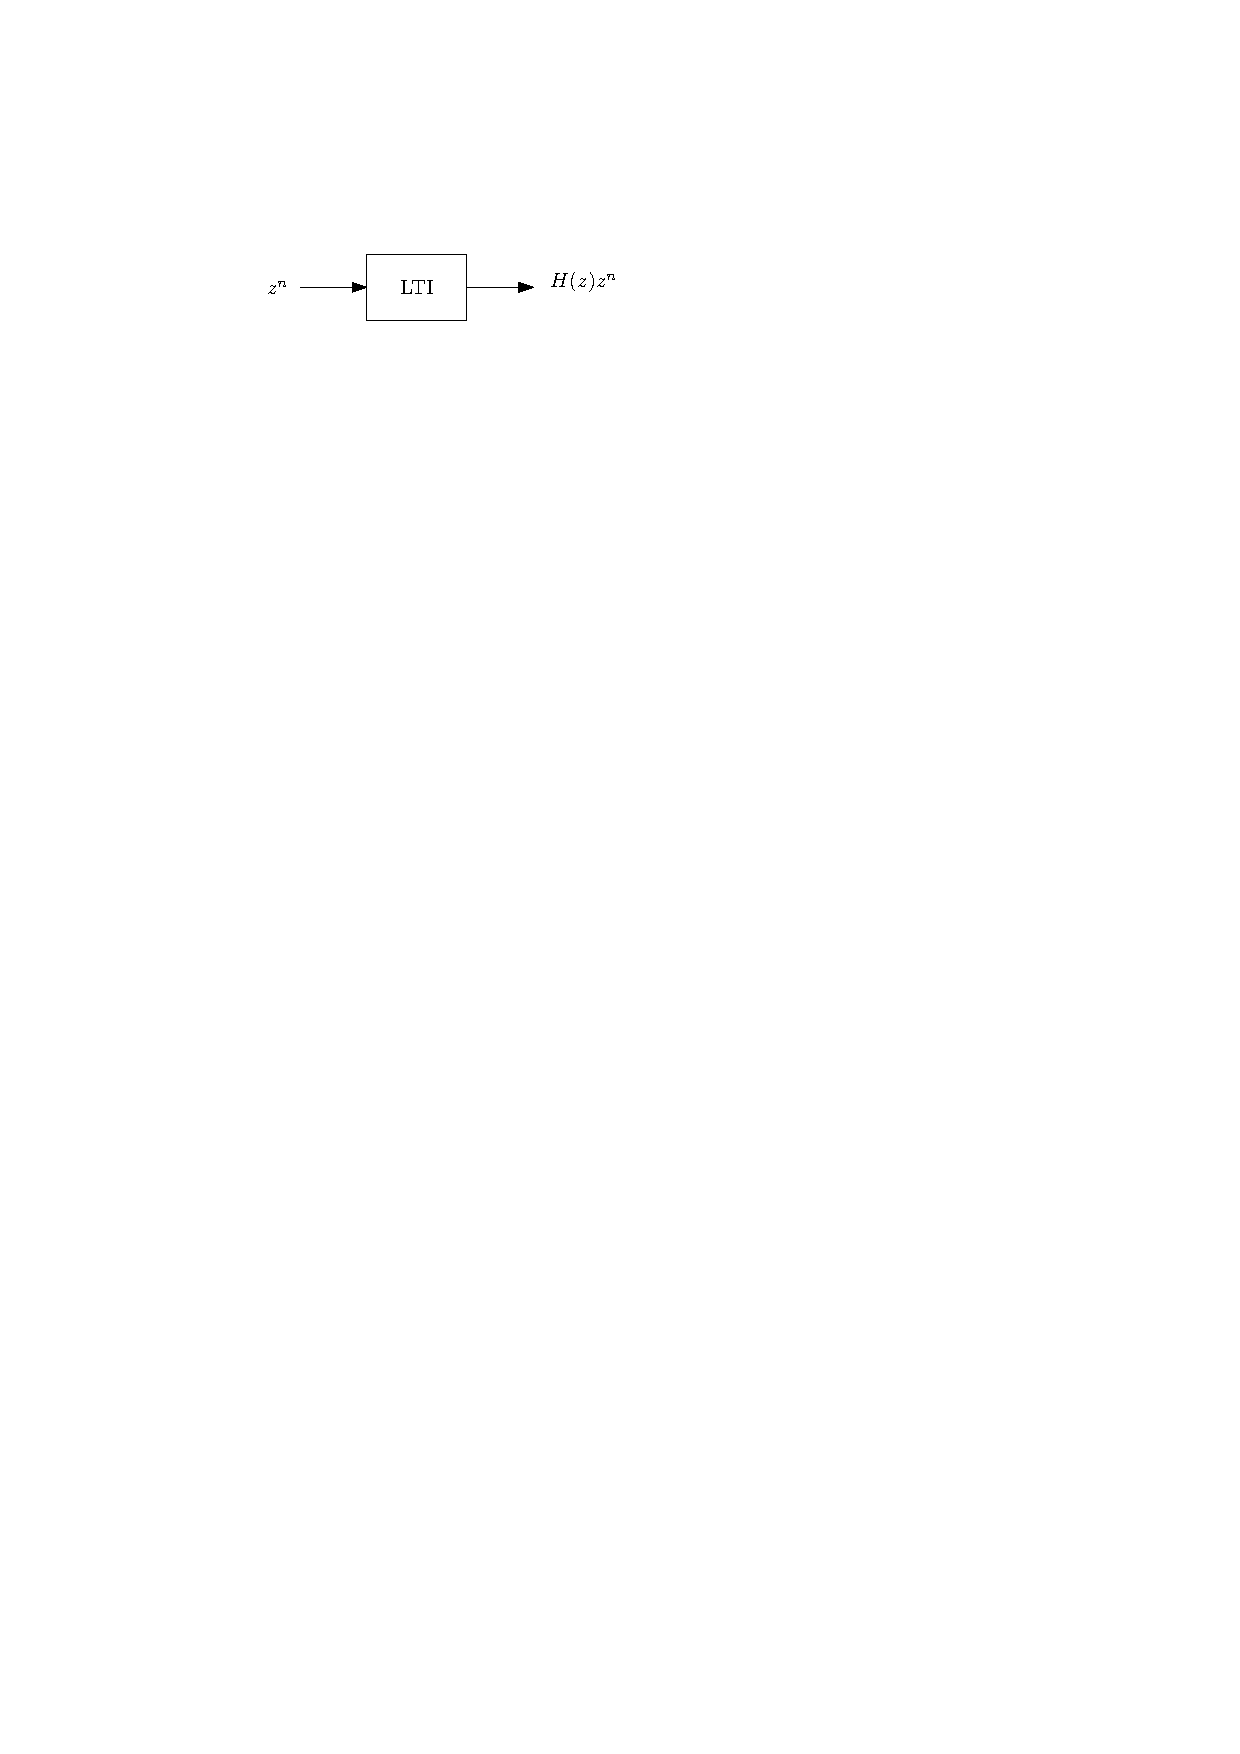
\includegraphics[scale=1]{graphics/19-dt-tf.pdf}
\end{center}

If a system is stable, then the region of convergence includes the unit circle $z = e^{j\omega}$. In that case, evaluating the Eigenvalues on the unit circle gives the DT frequency response $H\left(e^{j\omega}\right)$. This converts from a function of a complex variable, $z$, to one of a real variable $\omega$.

\begin{example} Consider a system with Eigenvalues (transfer function)
  \[
  H(z) = \frac{z}{z+\tfrac{1}{2}}\mbox{ for } |z| > \frac{1}{2}
  \]
  Determine the frequency response of the system, if possible.\\

  Solution: We first need to check if the system is stable using the region-of-convergence. Since the region of convergence includes the unit circle, the system is stable. To find the frequency response we substitute $s = e^{j\omega}$ to give
  \[
  H\left(e^{j\omega}\right) = \frac{e^{j\omega}}{e^{j\omega} + \tfrac{1}{2}}
  \]
  \\$\blacksquare$
\end{example}

\begin{example} Consider an apparently similar system with Eigenvalues
  \[
  H(z) = \frac{z}{z+2}\mbox{ for } |z| > 2
  \]
  Determine the frequency response of the system, if possible.\\

  Solution: Again, we first need to check of the system is stable using the region-of-convergence. Since the region of convergence does not include the unit circle, the system is unstable. Thus, the frequency response does not exist.
\\$\blacksquare$
\end{example}

\subsection*{Using the DTFT}

Another way we can view the frequency response is as the DT Fourier Transform of the impulse response. If the system is stable, then the impulse response is absolutely integrable, and the Fourier transform exists giving $H\left(e^{j\omega}\right) = \mathcal{F}\left\{h[n]\right\}$. This is connected to the transfer function by noting the bilateral Z transform and the DT Fourier Transform are identical under the substitution $z = e^{j\omega}$, which is allowed if the system is stable.

\begin{example} Suppose the impulse response of a DT LTI system is given by
  \[
  h[n] = \left(\frac{1}{4}\right)^n u[n] + 5\left(\frac{2}{3}\right)^n u[n] 
  \]
  Determine the frequency response of the system, if possible.\\

  Solution: If the system is stable, the Fourier transform of the impulse response exists. Since $\left(\frac{1}{4}\right) < 1$ and $\left(\frac{2}{3}\right) < 1$
  \[
H\left(e^{j\omega}\right) = \mathcal{F}\left\{ \left(\frac{1}{4}\right)^n u[n] + 5\left(\frac{2}{3}\right)^n u[n] \right\} = \mathcal{F}\left\{ \left(\frac{1}{4}\right)^n u[n]\right\} + 5 \mathcal{F}\left\{ \left(\frac{2}{3}\right)^n u[n] \right\} = \frac{e^{j\omega}}{e^{j\omega} - \left(\frac{1}{4}\right)} + \frac{5e^{j\omega}}{e^{j\omega} - \left(\frac{2}{3}\right)} 
\]\\
$\blacksquare$
\end{example}

\subsection*{Directly from a LCCDE}

By the convolution theorem of the DTFT, the frequency response is the ratio of the output to input in the frequency domain, i.e.
\[
H\left(e^{j\omega}\right) = \frac{Y\left(e^{j\omega}\right)}{X\left(e^{j\omega}\right)}
\]
We can easily determine this ratio from the LCCDE representation of the system using the shifting property of the DT Fourier Transform. Recall this property states if $\mathcal{F}\{x[n]\} = X\left(e^{j\omega}\right)$ then
\[
\mathcal{F}\left\{x[n-m] \right\} =  e^{-j\omega m} X\left(e^{j\omega}\right)\; .
\]
for index shift $m\in\mathbb{Z}$.

If the system is stable (and thus the frequency response exists) then \textbf{all} roots of the characteristic equation $Q(E)$ have magnitude that are less than one. If the system is stable we can take the Fourier transform of each term of the LCCDE using the shift property, then algebraically solve for the ratio of output to input. Note this provides a significant savings in analysis effort since we do not have to first find the impulse response, then take its Fourier transform to arrive at the frequency response (although that approach is still valid).

\begin{example} Consider a system described by the LCCDE
  \[
  3y[n+1]-y[n] = x[n+1]
  \]
  Determine the frequency response of the system, if possible.

  Solution: We first need to check for stability. The characteristic equation is $Q(E) = 3E - 1$ which has a single root of $\frac{1}{3}$. Since it is less than one, the system is stable. Next we take the Fourier transform of both sides and apply the derivative property
  \[
  3e^{j\omega} Y\left(e^{j\omega}\right) - Y\left(e^{j\omega}\right) = e^{j\omega} X\left(e^{j\omega}\right)
  \]
  and rearrange to get the frequency response
  \[
  H\left(e^{j\omega}\right) = \frac{e^{j\omega}}{3e^{j\omega}-1}
  \]\\
  $\blacksquare$
\end{example}

\section{Magnitude-phase representation of the DTFR}

Note that any complex valued function can be expressed in polar form using the magnitude and phase. Specifically the input and output can be put into this form
\[
X\left(e^{j\omega}\right) = |X\left(e^{j\omega}\right)|e^{\angle X\left(e^{j\omega}\right)}
\]
\[
Y\left(e^{j\omega}\right) = |Y\left(e^{j\omega}\right)|e^{\angle Y\left(e^{j\omega}\right)}
\]

By the convolution theorem then
  \[
  H\left(e^{j\omega}\right) = \frac{Y\left(e^{j\omega}\right)}{X\left(e^{j\omega}\right)} = \frac{|Y\left(e^{j\omega}\right)|e^{\angle Y\left(e^{j\omega}\right)}}{ |X\left(e^{j\omega}\right)|e^{\angle X\left(e^{j\omega}\right)}} = \frac{|Y\left(e^{j\omega}\right)|}{|X\left(e^{j\omega}\right)|}e^{\angle Y\left(e^{j\omega}\right) - \angle X\left(e^{j\omega}\right)} = |H\left(e^{j\omega}\right)|e^{\angle H\left(e^{j\omega}\right)}
  \]
  Thus we see that
  \[
  |H\left(e^{j\omega}\right)| = \frac{|Y\left(e^{j\omega}\right)|}{|X\left(e^{j\omega}\right)|}
  \]
  and
  \[
  \angle H\left(e^{j\omega}\right) = \angle Y\left(e^{j\omega}\right) - \angle X\left(e^{j\omega}\right)
  \]
  This is the magnitude and phase representation of the frequency response.
  
\section{DTFR acting on sinusoids}

The advantage of the magnitude and phase representation of the frequency response, is the ease with which we can find the output due to a sinusoidal input. If we apply a sinusoidal input $x[n] = A e^{j\omega n}$, the output is a the same sinusoid scaled by the frequency response $y[n] = H\left(e^{j\omega}\right) A e^{j\omega n}$.

\begin{center}
  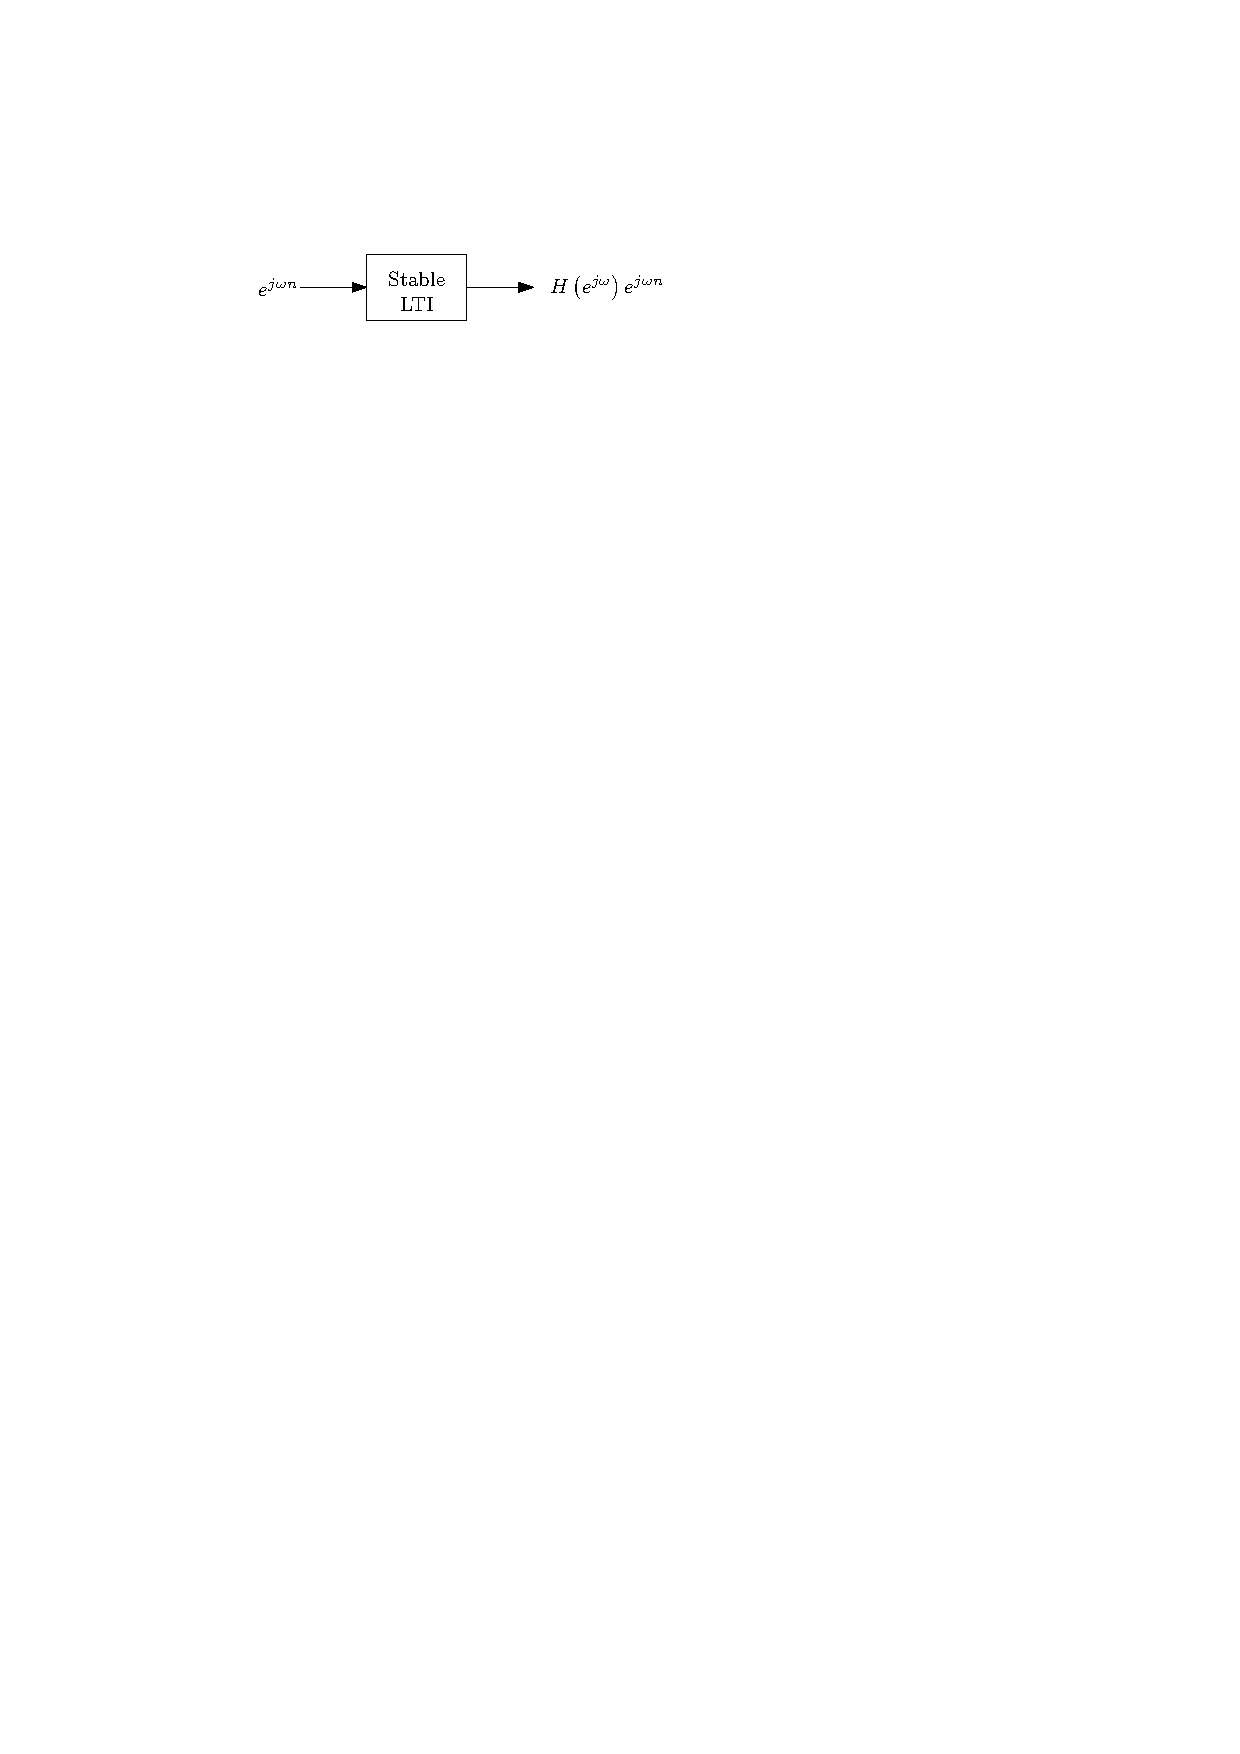
\includegraphics[scale=1]{graphics/19-dt-fr.pdf}
\end{center}

Now using the magnitude and phase representation
\[
y[n] = H\left(e^{j\omega}\right) A e^{j\omega n} = |H\left(e^{j\omega}\right)|e^{\angle H\left(e^{j\omega}\right)} A e^{j\omega n} = A |H\left(e^{j\omega}\right)| e^{j\omega n + \angle H\left(e^{j\omega}\right)} 
\]
Thus we can interpret the frequency response as telling us how the input sinusoids are scaled in magnitude and phase shifted as they pass through the system.

By the linearity property this extends to real sinusoidal inputs since
\begin{align*}
  x[n] &\longrightarrow y[n]\\
  \sin(\omega n) &\longrightarrow \frac{1}{2j}|H\left(e^{j\omega}\right)| e^{j\omega n + \angle H\left(e^{j\omega}\right)} - \frac{1}{2j}|H\left(e^{j\omega}\right)| e^{-j\omega n + \angle H\left(e^{j\omega}\right)}\\
  \sin(\omega n) &\longrightarrow |H\left(e^{j\omega}\right)|\sin(\omega n + \angle H\left(e^{j\omega}\right))  
\end{align*}
and
\begin{align*}
  x[n] &\longrightarrow y[n]\\
  \cos(\omega n) &\longrightarrow \frac{1}{2}|H\left(e^{j\omega}\right)| e^{j\omega n + \angle H\left(e^{j\omega}\right)} + \frac{1}{2}|H\left(e^{j\omega}\right)| e^{-j\omega n + \angle H\left(e^{j\omega}\right)}\\
  \cos(\omega n) &\longrightarrow |H\left(e^{j\omega}\right)|\cos(\omega n + \angle H\left(e^{j\omega}\right))  
\end{align*}

Also by the linearity property this analysis extends to the DT Fourier representation of a signal (an infinite sum of sinusoids):
\[
x[n] = \frac{1}{2\pi}\int\limits_{2\pi} X\left(e^{j \omega}\right) \, e^{j \omega n}\; d\omega \;\longrightarrow\; y[n] = \frac{1}{2\pi}\int\limits_{2\pi} H\left(e^{j \omega}\right) X\left(e^{j \omega}\right) \, e^{j \omega n}\; d\omega = \frac{1}{2\pi}\int\limits_{2\pi} \left| H\left(e^{j\omega}\right)\right| X\left(e^{j\omega}\right) \, e^{j \omega n + \angle H\left(e^{j\omega}\right)}\; d\omega
\]

Thus we arrive at the reason for the name DT \textit{Frequency Response} -- it specifies the response of a stable system to any linear combination of DT sinusoidal inputs, i.e. any signal with a Fourier Transform.

\section{Plotting the DT frequency response}

As in CT, we can visualize the frequency response as a plot of the real and imaginary part, or, of the magnitude and phase. Since the magnitude and phase allow us to directly see the system behavior at a given frequency, those plots are much more useful.

In contrast to CT, where the unique Bode plot format is used, for the DTFR it is most common to plot the magnitude spectrum in dB and the phase spectrum in rad over just $\omega = [0, \pi]$. Since the DTFR is periodic there is no need to compress the information using a logarithmic frequency scale. Further, if $x[n]$ is real the DTFR magnitude spectrum is even, so that the magnitude from $\omega = [\pi, 2\pi]$ is the same as from $\omega = [-\pi, 0]$. Also if $x[n]$ is real the DTFR phase spectrum is odd, so that the phase from $\omega = [\pi, 2\pi]$ is the same as the negative from $\omega = [-\pi, 0]$. Note we would not call this kind of plot a Bode plot as that is typically reserved for the CTFR.

As with the CTFR it is important to understand these plots well enough to create them on your own using software and read them.

\begin{example} Consider a frequency response given by
  \[
  H\left(e^{j\omega}\right) = \frac{4e^{j2\omega}}{4e^{j2\omega} - 1} 
  \]
  The following Matlab code shows you how to plot the spectrum (with some extra code to make it look nicer).
  
\begin{verbatim}
% compute the FTFR
w = 0:0.001:pi;
H = 4.*exp(j*2*w)./(4*exp(j*2*w) - 1);

% Create a nice DTFR plot 
hFig = figure();
hold on;

subplot(2,1,1);
hm = plot(w,20*log10(abs(H)));
axis tight;
grid on;
hTitle  = title ('Frequency Response');
hYLabel1 = ylabel('Magnitude (dB)');
set(gca, 'FontSize', 14, ...
    'Box', 'off', 'LineWidth', 2);

subplot(2,1,2);
hp = plot(w,angle(H));
axis tight;
grid on;
hYLabel2 = ylabel('Phase (radians)');
hXLabel = xlabel('Frequency (rad/sample)');
set(gca, 'FontSize', 14, 'Box', 'off', 'LineWidth', 2);

set(hm, 'linewidth', 2);
set(hp, 'linewidth', 2);
set([hXLabel, hYLabel1, hYLabel2]  , ...
     'FontSize'   , 14          );
set( hTitle                    , ...
     'FontSize'   , 14          , ...
     'FontWeight' , 'bold'      );
\end{verbatim}
This gives the following plot
\begin{center}
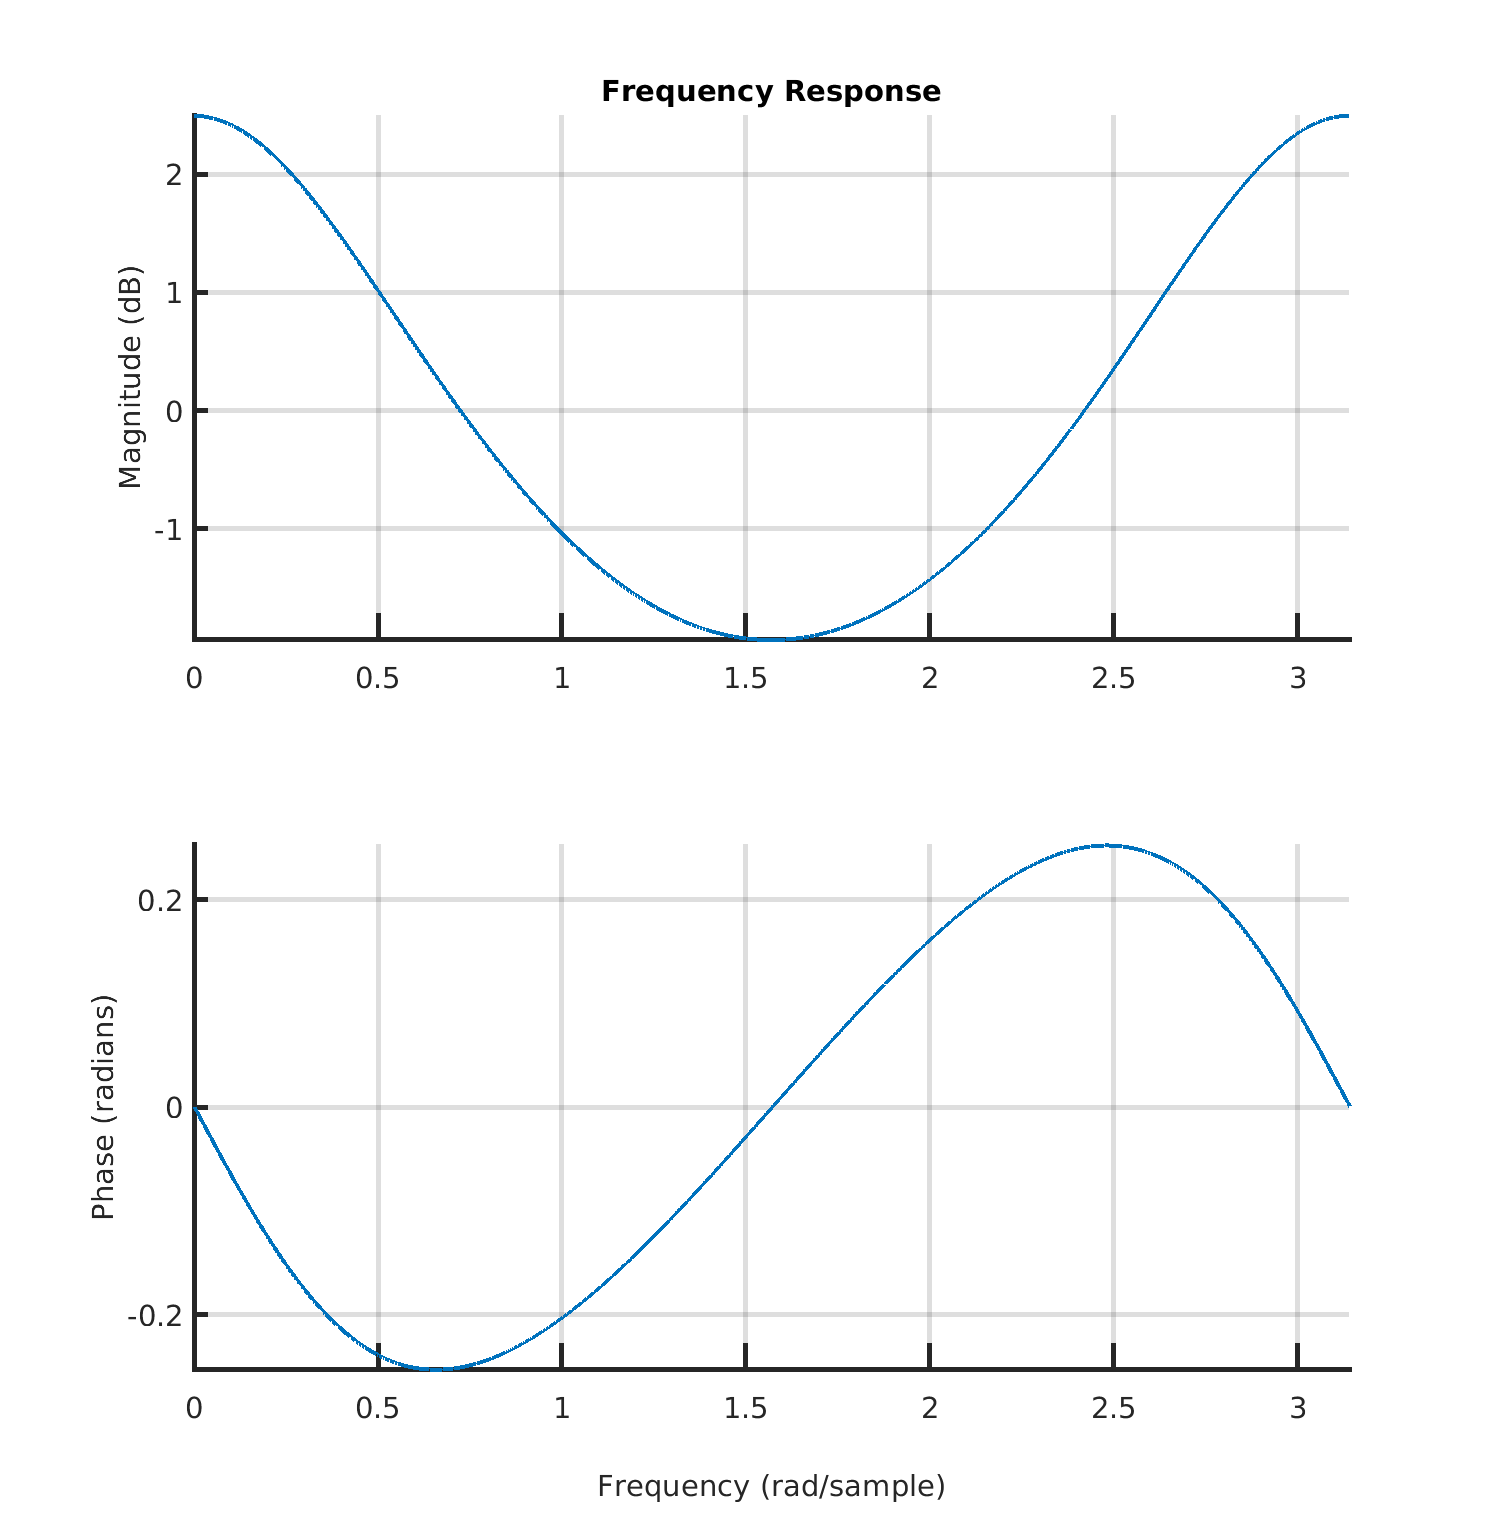
\includegraphics[scale=0.5]{graphics/lecture21_1.png}
\end{center}

$\blacksquare$
\end{example}

To read a Bode plot to see the behavior of the system at a given frequency, one need only read the values off the plot and convert from dB to a unit-less gain.

\begin{example}
  Suppose you are given the DTFR plot (only) from the previous example and are asked: what the output of the system is when the input is $x[n] = \cos\left(\frac{\pi}{4} n\right)$?\\
  \textbf{Solution:} We go to the frequency $\frac{\pi}{4} \approx 0.78$ on the plot and read off a value of about $-0.1$ dB for the magnitude and about $-0.25$ rad for the phase. To convert back from dB
  \[
  \left|H\left(e^{j\frac{\pi}{4}}\right)\right| = 10^{\frac{-0.1}{20}} \approx 0.988 
  \]
  so the output would be
  \[
  y[n] \approx 0.988\cos\left(\frac{\pi}{4} n  - 0.25\right)
  \]
  $\blacksquare$
\end{example}
